% !TeX root = ../solution.tex

\hypertarget{he22.06}{%
\chapter{[HE22.06] Fibonacci Rabbits}\label{he22.06}}

\begin{marginfigure}
	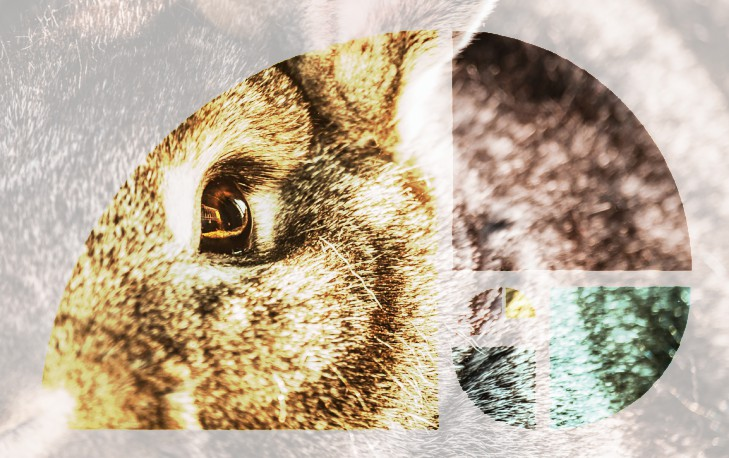
\includegraphics[width=49mm]{level3/challenge6.jpg}
\end{marginfigure}
\subsection{Intro}
Everyone loves rabbits!

\noindent\url{http://46.101.107.117:2201}

\noindent
Note: The service is restarted every hour at x:00.
  

\section{Solution}\label{hv21.06-solution}

Looking at the source code of the page, we see a list of images to be
displayed:

\noindent\begin{fullwidth}
{\footnotesize\begin{verbatim}
<div><img src="images/rabbit-17711.jpg" /><a href="#">Petal</a></div>
<div><img src="images/rabbit-75025.jpg" /><a href="#">Harley</a></div>
<div><img src="images/rabbit-34.jpg" /><a href="#">Rosie</a></div>
<div><img src="images/rabbit-987.jpg" /><a href="#">Petunia</a></div>
<div><img src="images/rabbit-8.jpg" /><a href="#">Mortimer</a></div>
<div><img src="images/rabbit-1.jpg" /><a href="#">Henry</a></div>
<div><img src="images/rabbit-144.jpg" /><a href="#">Miffy</a></div>
<div><img src="images/rabbit-2584.jpg" /><a href="#">E.B.</a></div>
<div><img src="images/rabbit-89.jpg" /><a href="#">Baxter</a></div>
<div><img src="images/rabbit-55.jpg" /><a href="#">Archie</a></div>
<div><img src="images/rabbit-5.jpg" /><a href="#">Murphy</a></div>
<div><img src="images/rabbit-317811.jpg" /><a href="#">Doc</a></div>
<div><img src="images/rabbit-2.jpg" /><a href="#">Hopper</a></div>
<div><img src="images/rabbit-6765.jpg" /><a href="#">Fluffy</a></div>
<div><img src="images/rabbit-46368.jpg" /><a href="#">Daffodil</a></div>
<div><img src="images/rabbit-28657.jpg" /><a href="#">Buttons</a></div>
<div><img src="images/rabbit-233.jpg" /><a href="#">Freddie</a></div>
<div><img src="images/rabbit-1597.jpg" /><a href="#">Roger</a></div>
<div><img src="images/rabbit-514229.jpg" /><a href="#">Bucky</a></div>
<div><img src="images/rabbit-4181.jpg" /><a href="#">Oliver</a></div>
<div><img src="images/rabbit-13.jpg" /><a href="#">Olive</a></div>
<div><img src="images/rabbit-3.jpg" /><a href="#">Bugs</a></div>
<div><img src="images/rabbit-377.jpg" /><a href="#">Flower</a></div>
<div><img src="images/rabbit-10946.jpg" /><a href="#">Chester</a></div>
<div><img src="images/rabbit-610.jpg" /><a href="#">Bubbles</a></div>
<div><img src="images/rabbit-121393.jpg" /><a href="#">Coco</a></div>
<div><img src="images/rabbit-21.jpg" /><a href="#">Clover</a></div>
\end{verbatim}
}
\end{fullwidth}

\noindent
The file names have an numbering that follows the Fibonacci series, so ordering
them by the number shows that the file \verb+rabbit-196418.jpg+ is missing.
Have a look at it\\
\noindent\verb+he2022{th1z_41nT_4_r4bB1T!}+

\begin{marginfigure}
	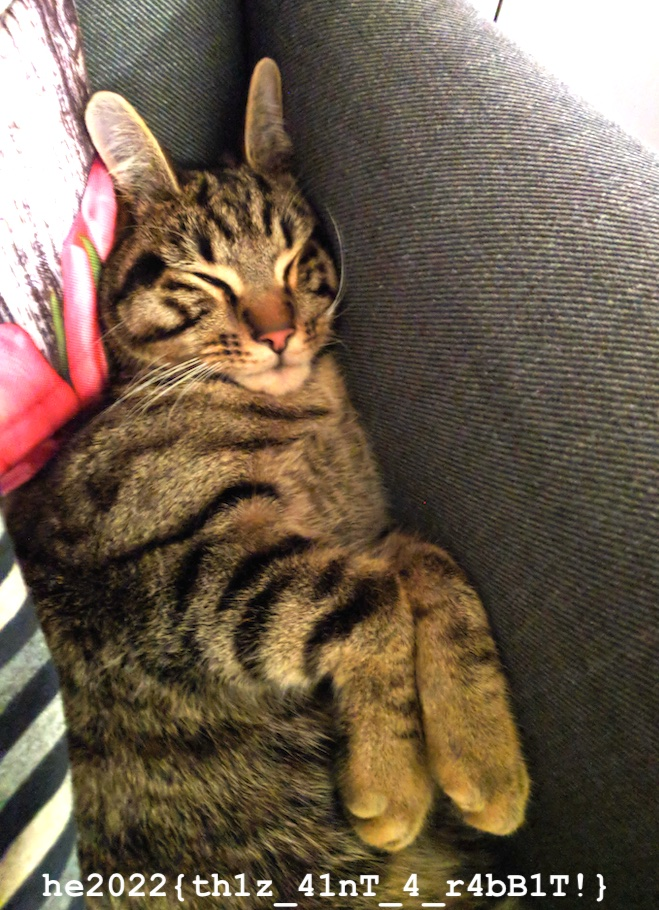
\includegraphics[width=50mm]{level3/rabbit-196418.jpg}
\end{marginfigure}



